\documentclass[12pt, titlepage]{article}

\usepackage{fullpage}
\usepackage[round]{natbib}
\usepackage{multirow}
\usepackage{booktabs}
\usepackage{tabularx}
\usepackage{graphicx}
\usepackage{float}
\usepackage{hyperref}


\hypersetup{
    colorlinks,
    citecolor=blue,
    filecolor=black,
    linkcolor=red,
    urlcolor=blue
}

%% Comments
\usepackage{color}
\newif\ifcomments\commentstrue %displays comments
%\newif\ifcomments\commentsfalse %so that comments do not display
\ifcomments
\newcommand{\authornote}[3]{\textcolor{#1}{[#3 ---#2]}}
\newcommand{\todo}[1]{\textcolor{red}{[TODO: #1]}}
\else
\newcommand{\authornote}[3]{}
\newcommand{\todo}[1]{}
\fi
\newcommand{\wss}[1]{\authornote{blue}{SS}{#1}} 
\newcommand{\plt}[1]{\authornote{magenta}{TPLT}{#1}} %For explanation of the template
\newcommand{\an}[1]{\authornote{cyan}{Author}{#1}}
%% Common Parts
\newcommand{\progname}{4TB6 - Mechatronics Capstone} % PUT YOUR PROGRAM NAME HERE
\newcommand{\authname}{Team \#5, Locked \& Loaded
\\ Abi Nevo, nevoa
\\ Elsa Bassi, bassie
\\ Steffi Ralph, ralphs1
\\ Abdul Iqbal, iqbala18
\\ Stephen De Jong, dejons1
\\ Anthony Shenouda, shenoa2} % AUTHOR NAMES                  

\usepackage{hyperref}
    \hypersetup{colorlinks=true, linkcolor=blue, citecolor=blue, filecolor=blue,
                urlcolor=blue, unicode=false}
    \urlstyle{same}


\newcounter{acnum}
\newcommand{\actheacnum}{AC\theacnum}
\newcommand{\acref}[1]{AC\ref{#1}}

\newcounter{ucnum}
\newcommand{\uctheucnum}{UC\theucnum}
\newcommand{\uref}[1]{UC\ref{#1}}

\newcounter{mnum}
\newcommand{\mthemnum}{M\themnum}
\newcommand{\mref}[1]{M\ref{#1}}

\begin{document}

\title{System Design for \progname{}} 
\author{\authname}
\date{\today}

\maketitle

\pagenumbering{roman}

\section{Revision History}

\begin{tabularx}{\textwidth}{p{3cm}p{2cm}X}
\toprule {\bf Date} & {\bf Version} & {\bf Developer}\\
\midrule
January 16, 2023 & 1.0 & Steffi\\
\bottomrule
\end{tabularx}

\newpage

\section{Reference Material}

This section records information for easy reference.

\subsection{Abbreviations and Acronyms}

\renewcommand{\arraystretch}{1.2}
\begin{tabular}{l l} 
  \toprule		
  \textbf{symbol} & \textbf{description}\\
  \midrule 
  SRS & Software Requirements Specification\\
  FR & Functional Requirements\\
  NFR & Nonfunctional Requirements\\
  LC & Likely Changes\\
  ULC & Unlikely Changes\\
  SC & System Contraints\\
  A & Assumptions\\
  MV & Monitored Variables\\
  \bottomrule
\end{tabular}\\

\newpage

\tableofcontents

\newpage

%\listoftables

\listoffigures

\newpage

\pagenumbering{arabic}

\section{Introduction}

For more information on the project breakdown, planning or delivery refer to the following documentation:
 \href{https://github.com/NevoAbigail/Capstone/blob/main/docs/ProblemStatementAndGoals/ProblemStatement.pdf}{Problem Statement and Goals},
 \href{https://github.com/NevoAbigail/Capstone/blob/main/docs/DevelopmentPlan/DevelopmentPlan.pdf}{Development Plan},
 \href{https://github.com/NevoAbigail/Capstone/blob/main/docs/SRS/SRS.pdf}{SRS},
 \href{https://github.com/NevoAbigail/Capstone/blob/main/docs/HazardAnalysis/HazardAnalysis.pdf}{HA},
 \href{https://github.com/NevoAbigail/Capstone/blob/main/docs/Design/SoftArchitecture/MG.pdf}{MG},
 \href{https://github.com/NevoAbigail/Capstone/blob/main/docs/Design/SoftDetailedDes/MIS.pdf}{MIS}.
%\wss{Include references to your other documentation}

\section{Purpose}
The purpose of this documentation is to break down all of the components that will come together to create the final product, as well as how they interact and why they are used. This document will show everything that the SmartLock is made from and when it will be assembled in order to provide transparency throughout the entire design project.

%\wss{Purpose of your design documentation}

%\wss{Point to your other design documents}

\section{Scope}

This lock and application are designed for the use of the average bike rider. It is simple and easy to use and locks the primary components of the bike so that the user can be confident in its security. 

 \begin{figure}[h!]
 \begin{center}
 {
  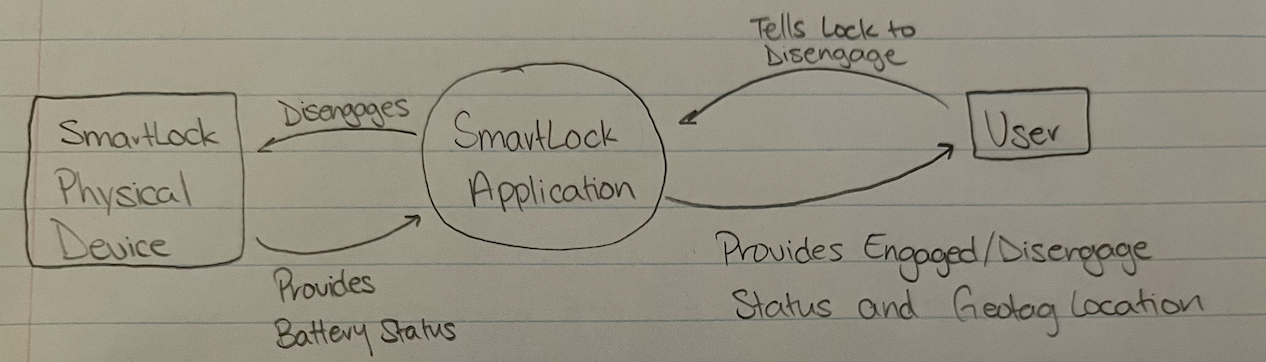
\includegraphics[width=0.9\linewidth]{System Context.png}
 }
 \caption{\label{System Context} System Context}
 \end{center}
 \end{figure}


%\wss{Include a figure that show the System Context (showing the boundary betweenyour system and the environment around it.)}

\section{Project Overview}

\subsection{Normal Behaviour}

The normal behaviour that is expected with the SmartLock is multistep:
\begin{enumerate}
\item After the first purchase of the SmartLock the user will have to attach the lock to the bike, and download the application from the AppStore or Google Play and pair the application with the physical device (this only happens once)
\item The user will put the cable around the wheel and external frame and then push the pin into the locking hole
\item The user will be able to geotag the location of the locked bike on the application
\item The user will be able to disengage the lock on the application so that they can remove the pin from the hole and release the bike
\item The application will warn the user when there is low battery so that the lock can be recharged
\end{enumerate}

\subsection{Undesired Event Handling}

In the case of an undesired or unexpected event, the lock will stay in the locked position and the application will block the unlocking process. While this does inhibit the user's ability to be able to use their bike, it does prevent the bike from being stolen which is more important in an uncertain situation. The user will be able to reset the lock to eliminate the stimulus that caused the event and be able to use their app as normal after.

%\wss{How you will approach undesired events}

\subsection{Component Diagram}

 \begin{figure}[h!]
 \begin{center}
 {
  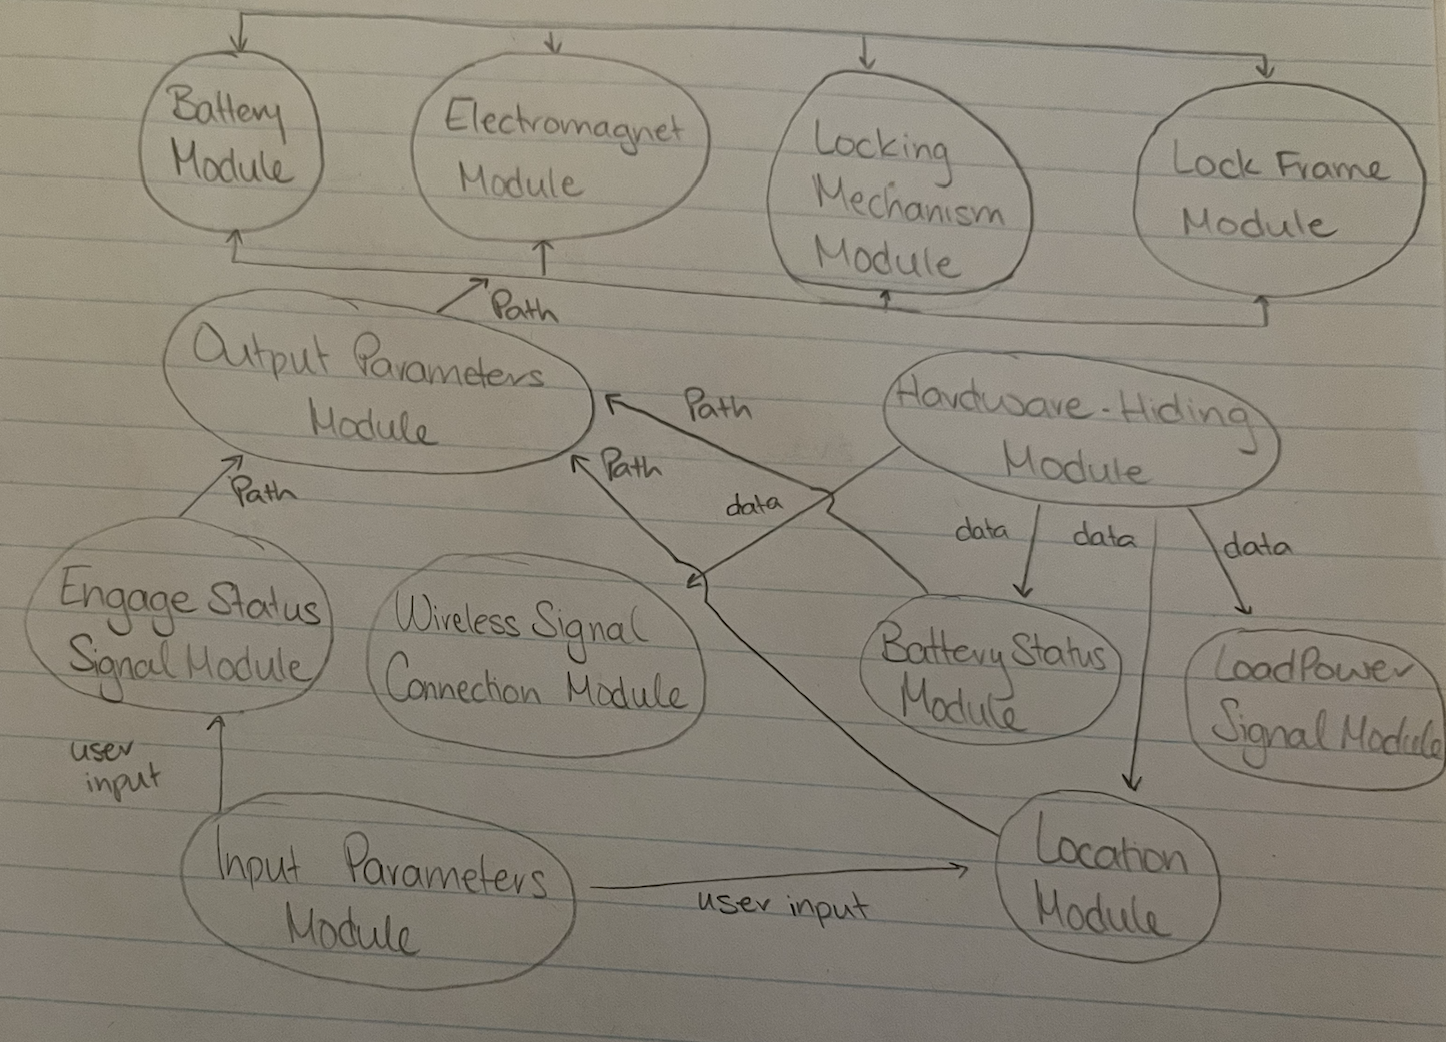
\includegraphics[width=0.8\linewidth]{component diagram.png}
 }
 \caption{\label{component diagram} Component Diagram}
 \end{center}
 \end{figure}

\subsection{Connection Between Requirements and Design} %\label{SecConnection}

\begin{minipage}{\textwidth}
\renewcommand*{\arraystretch}{1.5}
\begin{tabular}{| p{0.48\textwidth} | p{0.52\textwidth} | }
 \hline
 Requirement/Constraint & Design Description\\ 
 \hline
 SC2:  The materials and resources used to design and build the project must be accessible to students& Rev 0 will be primarily made from 3D printed materials, with an option to move to machining for Rev 1\\
 \hline
 SC4:  The project must be mounted on existing bike designs & Current market bike lock mount is being used to ensure compatibility\\
 \hline
 SC5:  The project must be locked on existing external locking frames or racks &Current market bike lock cable is being used to ensure compatibility\\
 \hline
FR2: LockDisengage input must disengage the lock on the bike & Using an electromagnet for locking allows for a easier connection to a microcontroller that can communicate with a phone app\\
 \hline
FR3,4,7: The application has to show the status of the electromagnet and battery as well as display the location&The UI was designed so that this information is easy to see, these are requirements to make the lock secure but they relate to the user experience\\
 \hline
FR8: Effective Bike Lock: The lock is sturdy and cannot be manually opened by the average human once engaged& Using simple pieces without a lot of components that can break off makes it more sturdy, and using a market bike cable makes sure it is strong enough not to be broken\\
 \hline
FR9: Lock must only be engaged/disengaged by the intended user(s)& The application is password protected\\
 \hline
NFR1: Can be used by people of any language&Language choice can be selected on the app\\
 \hline
NFR2, 12: Can reasonably be used without instructions or extra force& Uses similar mechanics of inserting a pin that traditional bike locks use\\
 \hline
NFR5: The design must not impede normal bike functions& Attaches to the bike using current market mounts so that it is small and out of the way\\
 \hline
NFR6,7: The lock must be waterproofed to withstand normal rainfall & All circuitry is encased and the materials are waterproof\\
 \hline
NFR11: iPhone app locking must be quicker to use than a typical keyed/combo bike lock &The phone will accept face or touch id as a password form and then one button click will unlock the bike \\
 \hline
NFR14: Batteries must be accessible to replace or chargeable&A chargeable battery was used for user ease and less waste\\
 \hline
NFR22: The app should run on iOS and Android.&Designed on Flutter for cross-platform development\\
 \hline
\end{tabular}
\end{minipage}\\


\wss{The intention of this section is to document decisions that are made
  ``between'' the requirements and the design.  To satisfy some requirements,
  design decisions need to be made.  Rather than make these decisions implicit,
  they are explicitly recorded here.  For instance, if a program has security
  requirements, a specific design decision may be made to satisfy those
  requirements with a password.}

\newpage
\section{System Variables}

%\wss{Include this section for Mechatronics projects}

\subsection{Monitored Variables}

\begin{minipage}{\textwidth}
\renewcommand*{\arraystretch}{1.5}
\begin{tabular}{| p{0.23\textwidth} | p{0.54\textwidth} | p{0.08\textwidth} | p{0.15\textwidth} |}
 \hline
 Variable Name & Description & Type & Units \\ 
 \hline
 m\_SignalEngaged & Monitors whether or not the locking mechanism is engaged & Digital & Boolean \\ 
  \hline
 m\_SignalDisengaged & Monitors whether or not the locking mechanism is disengaged & Digital & Boolean \\ 
  \hline
 m\_SignalClosed& Monitors whether or not the physical mechanism is closed & Digital & Boolean \\ 
  \hline
 m\_Location & Monitors the location of the bike when it is locked & Analog & Coordinates \\ 
  \hline
 m\_BatteryPower & Monitors the current battery percentage & Analog & Percentage \\ 
 \hline
\end{tabular}
\end{minipage}\\

\subsection{Controlled Variables}

\begin{minipage}{\textwidth}
\renewcommand*{\arraystretch}{1.5}
\begin{tabular}{| p{0.25\textwidth} | p{0.52\textwidth} | p{0.08\textwidth} | p{0.15\textwidth} |}
 \hline
 Variable Name & Description & Type & Units \\ 
 \hline
 c\_LockEngaged & Engages the lock & Digital & Boolean \\ 
  \hline
 c\_LocklDisengaged & Disengages the lock & Digital & Boolean \\ 
  \hline
 c\_LockClosed& Indicates to the user that the latch is closed & Digital & Boolean \\ 
  \hline
 c\_BikePosition & Marks the location of the bike when it is locked & Analog & Coordinates \\ 
  \hline
 c\_BatteryPercentStatus & Indicates what the percentage of the battery is & Analog & Percentage \\ 
 \hline
\end{tabular}
\end{minipage}\\

\subsection{Constants Variables - NA}

\newpage
\section{User Interfaces}
There are two user interfaces related to our product. The first is through an application (SmartLock) and the second is the lock itself where the user will be required to manually open/close the chain to secure the bike. \\


The application is where the user will be able to disengage their lock and locate where it was left with the Geotagging feature. \\

 \begin{figure}[h!]
 \begin{center}
 {
  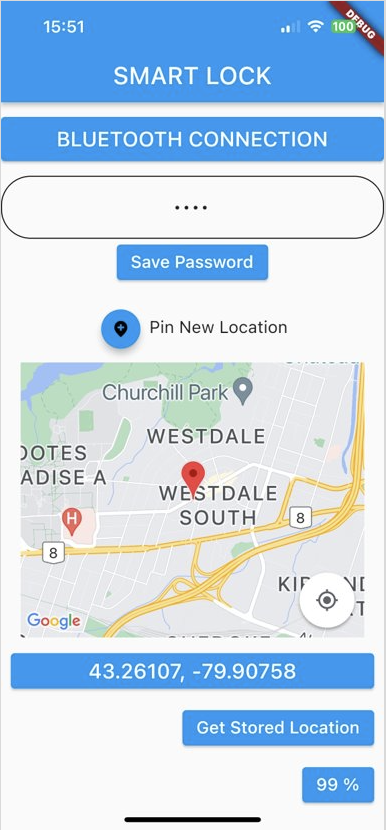
\includegraphics[width=0.5\linewidth]{UI.png}
 }
 \caption{\label{Application User Interface} Application User Interface}
 \end{center}
 \end{figure}

\newpage
The hardware will be mounted to the bike, which will require user interaction upon the purchase of the SmartLock. Additionally, the user must push the locking pin into the hole to engage the lock, and disengage the lock with their phone to be able to remove the pin. 

 \begin{figure}[h!]
 \begin{center}
 {
  \includegraphics[width=0.9\linewidth]{HardwareUI.png}
 }
 \caption{\label{Hardware User Interface} Hardware User Interface}
 \end{center}
 \end{figure}

%\wss{Design of user interface for software and hardware.  Attach an appendix if needed. Drawings, Sketches, Figma}

\section{Design of Hardware}

The following is a list of the hardware components that will be acquired to build the SmartLock:
\begin{itemize}
\item Arduino
\item Locking Cable
\item Bike Attachment
\end{itemize}

The following is a list of the hardware components that will be built for the SmartLock:
\begin{itemize}
\item Circuit (discussed below)
\item Lock Housing (CAD)
\item Locking Mechanism (CAD)
\end{itemize}

See Appendix for hardware components both purchased and 3D printed

%\wss{Most relevant for mechatronics projects}
%\wss{Show what will be acquired}
%\wss{Show what will be built, with detail on fabrication and materials}
%\wss{Include appendices as appropriate, possibly with sketches, drawings, CAD, etc}

\section{Design of Electrical Components}

The following is a list of the electrical components that will be used in combination with the aforementioned Arduino to make up the circuitry used to control the SmartLock:
\begin{itemize}
\item Battery
\subitem - Needs to be acquired
\item Transistor
\subitem - Previously owned
\item Wiring
\subitem - Previously owned
\item Magnet
\subitem - Needs to be acquired
\item Charging board (maybe)
\subitem - Needs to be acquired
\item Resistors (maybe)
\subitem - Previously owned
\end{itemize}

See the Appendix for visualizations of the components and circuit diagrams

%\wss{Most relevant for mechatronics projects}
%\wss{Show what will be acquired}
%\wss{Show what will be built, with detail on fabrication and materials}
%\wss{Include appendices as appropriate, possibly with sketches, drawings, circuit diagrams, etc}

\section{Design of Communication Protocols}

In order for the SmartLock to work there are signals that have to be used to communicate between the application and the physical lock. 
The features of our lock include: 
\begin{itemize}
\item Locking the bike from the application
\subitem - A Bluetooth microcontroller is utilized so that the application is able to communicate with the physical device
\subitem - The microcontroller is wired directly to an electromagnet that controls the disengagement of the lock
\item Geotagging the location of the bike
\subitem - Integration with Google Maps will be used to save the coordinates of the locked bike
\end{itemize}
%\wss{If appropriate}

\section{Timeline}

\begin{minipage}{\textwidth}
\renewcommand*{\arraystretch}{1.5}
\begin{tabular}{| p{0.12\textwidth} | p{0.38\textwidth} | p{0.50\textwidth} |}
 \hline
 Date & Description & Group Member Assigned\\ 
 \hline
 January 16 & Housing Design & Abi, Elsa \& Steffi\\ 
 \hline
 January 18 & Design Documentation & MG - Elsa \newline MIS - Abi \& Anthony \newline SystDes - Steffi\\ 
  \hline
  January 22 & CAD of Housing Design & Steffi\\ 
  \hline
    January 22 & Circuit & Stephen\\ 
  \hline
    January 22 & App & Anthony\\ 
    \hline
    January 22 & Arduino Coded & Abi\\ 
  \hline
   January 25 & Arduino and Circuit Testing & Abi \& Stephen\\ 
  \hline
   January 29 & Housing 3D Printed & Abdul\\ 
  \hline
    February 1& Assemble Housing and Circuit & Steffi \& Stephen\\ 
  \hline
   February 1& All Documentation has been updated to reflect the current project including Git issues \& battery calculations& Elsa\\ 
  \hline
      February 4 & Rev 0 Testing & Everyone\\ 
  \hline
  February 6 & Rev 0 Demonstration & App \& Arduino - Anthony \& Abi \newline Circuit - Stephen \newline Housing - Steffi \& Elsa \newline Documentation Elsa \& Steffi\\
  \hline
  March 8 & V \& V Report Rev 0 & Everyone \newline(Reqs divided by area of expertise on Rev 0 Demonstration)\\
  \hline
 March 20 & Final Demonstration & Everyone \newline(Divided by areas of work)\\
 \hline
 April 5 & Final Documentation & Everyone \newline(Divided by areas of work)\\
 \hline
 TBD & EXPO & Everyone (Divided by areas of work)\\
 \hline
\end{tabular}
\end{minipage}\\

%\wss{Schedule of tasks and who is responsible}

% \bibliographystyle {plainnat}
% \bibliography{../../../refs/References}

\newpage{}
\section{Appendix}

\subsection{Interface - Included in Section 8}

%\wss{Include additional information related to the appearance of, and interaction with, the user interface}

\subsection{Mechanical Hardware}

 \begin{figure}[ht]
 \begin{center}
 {
  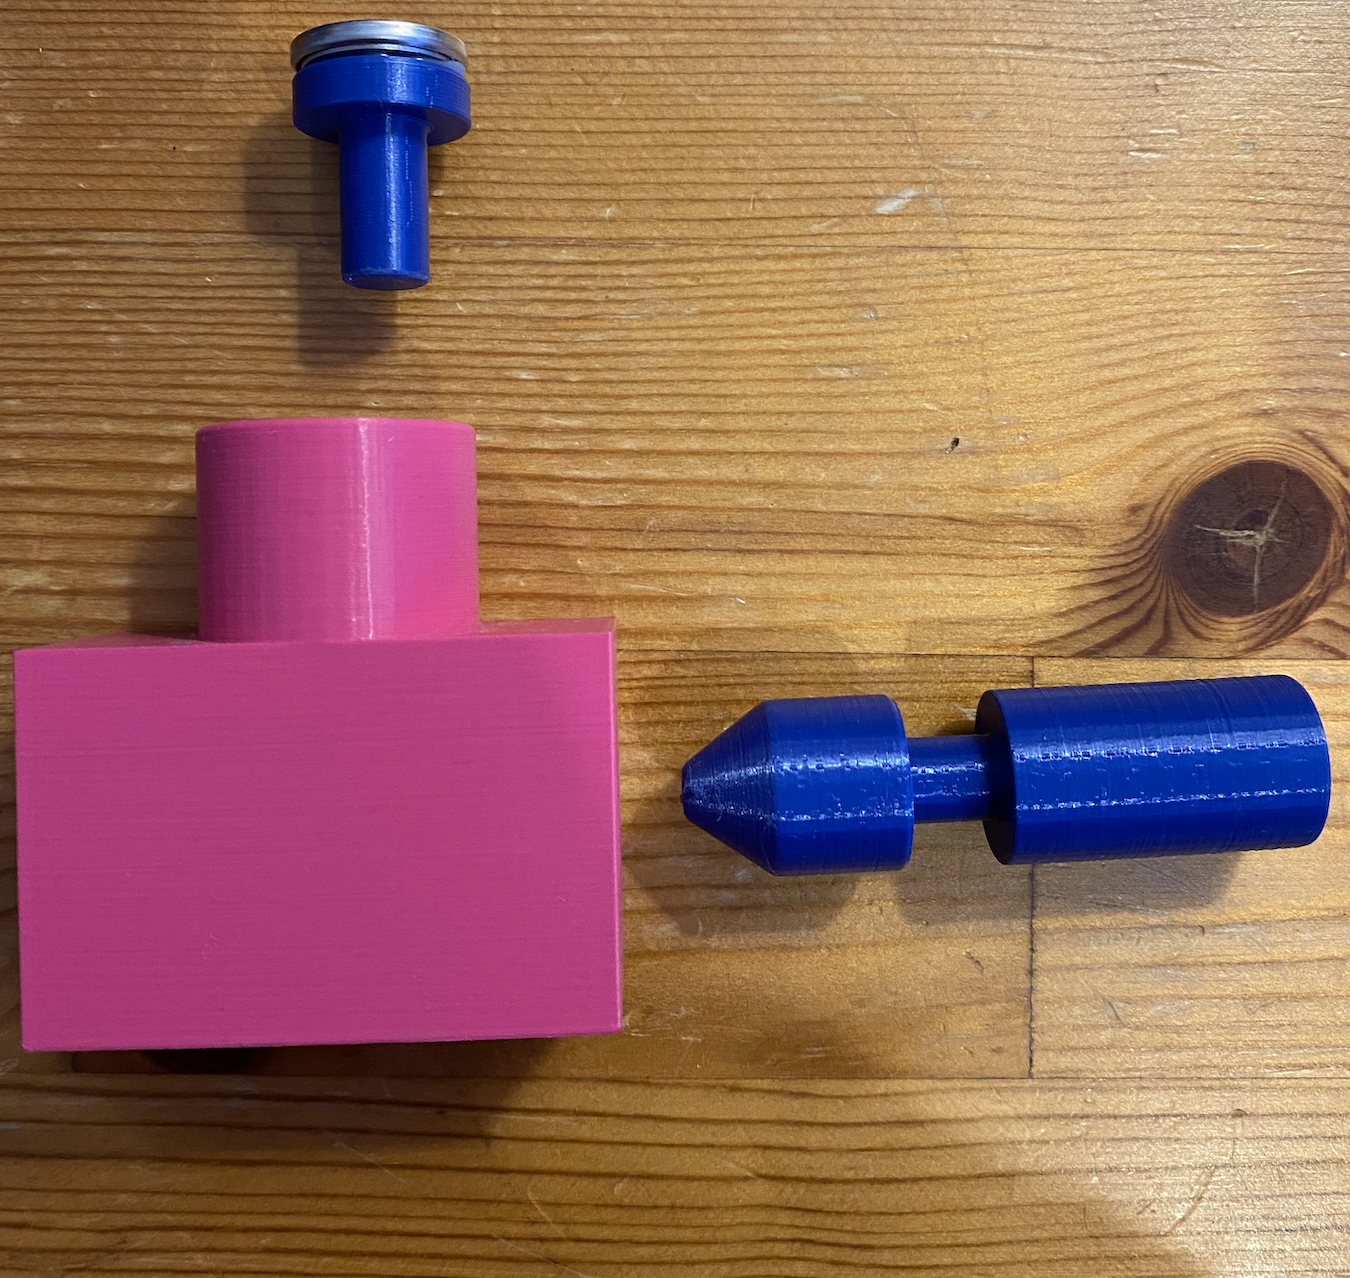
\includegraphics[width=0.4\linewidth]{1.png}
  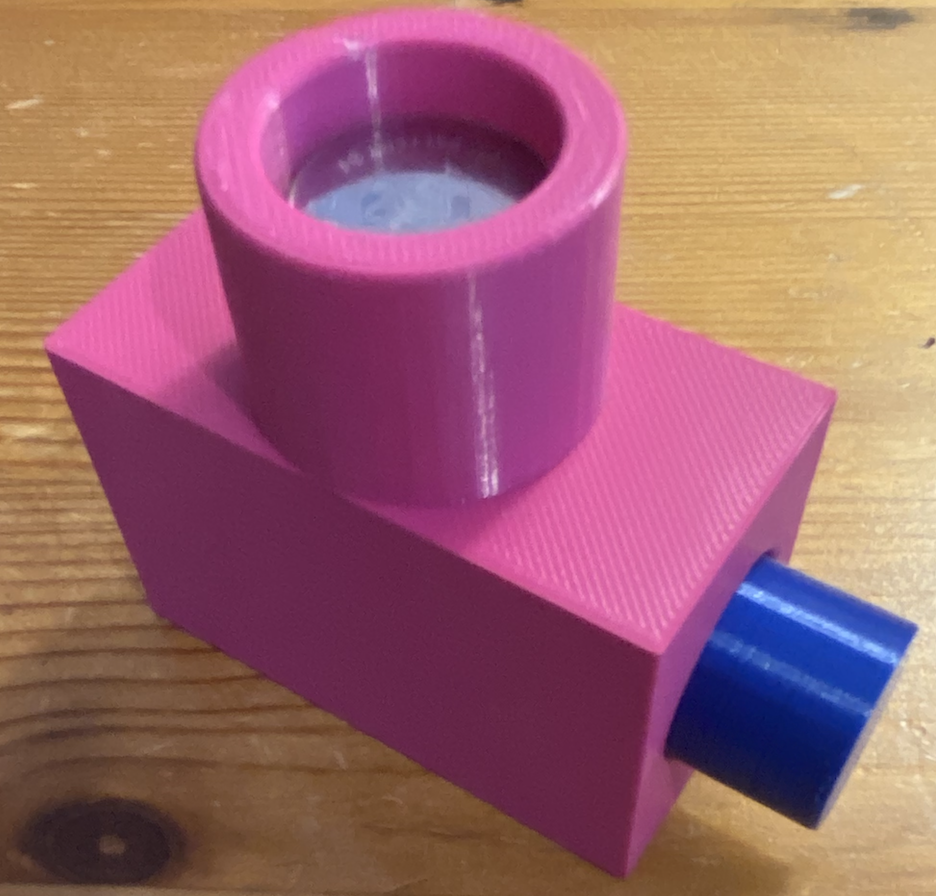
\includegraphics[width=0.4\linewidth]{2.png}
 }
 \caption{\label{Locking Mechanism Components} Locking Mechanism Components Disassembled and Assembled}
 \end{center}
 \end{figure}
 
  \begin{figure}[ht]
 \begin{center}
 {
  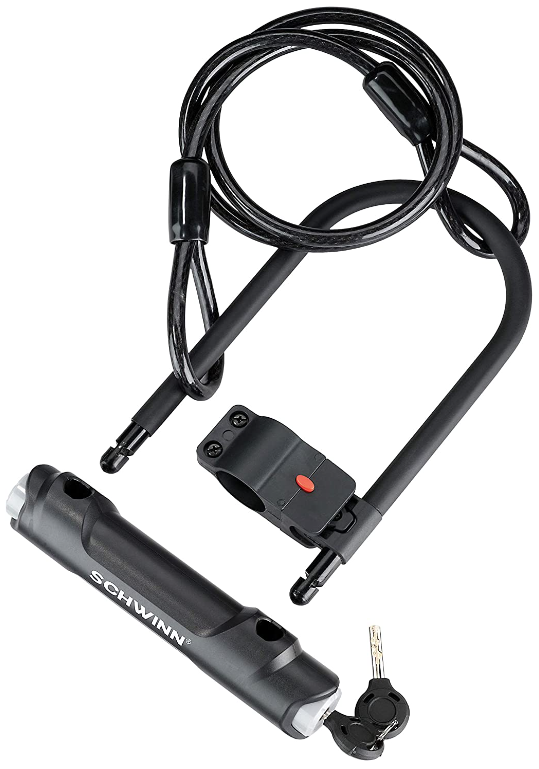
\includegraphics[width=0.2\linewidth]{BikeLock.png}
 }
 \caption{\label{BikeLock} Bike Lock Cable and Mount Attachment}
 \end{center}
 \end{figure}
 
 \begin{figure}[ht]
 \begin{center}
 {
  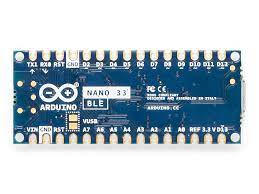
\includegraphics[width=0.3\linewidth]{arduino.png}
 }
 \caption{\label{Arduino} Arduino}
 \end{center}
 \end{figure}
 \newpage

\subsection{Electrical Components}

 \begin{figure}[ht]
 \begin{center}
 {
  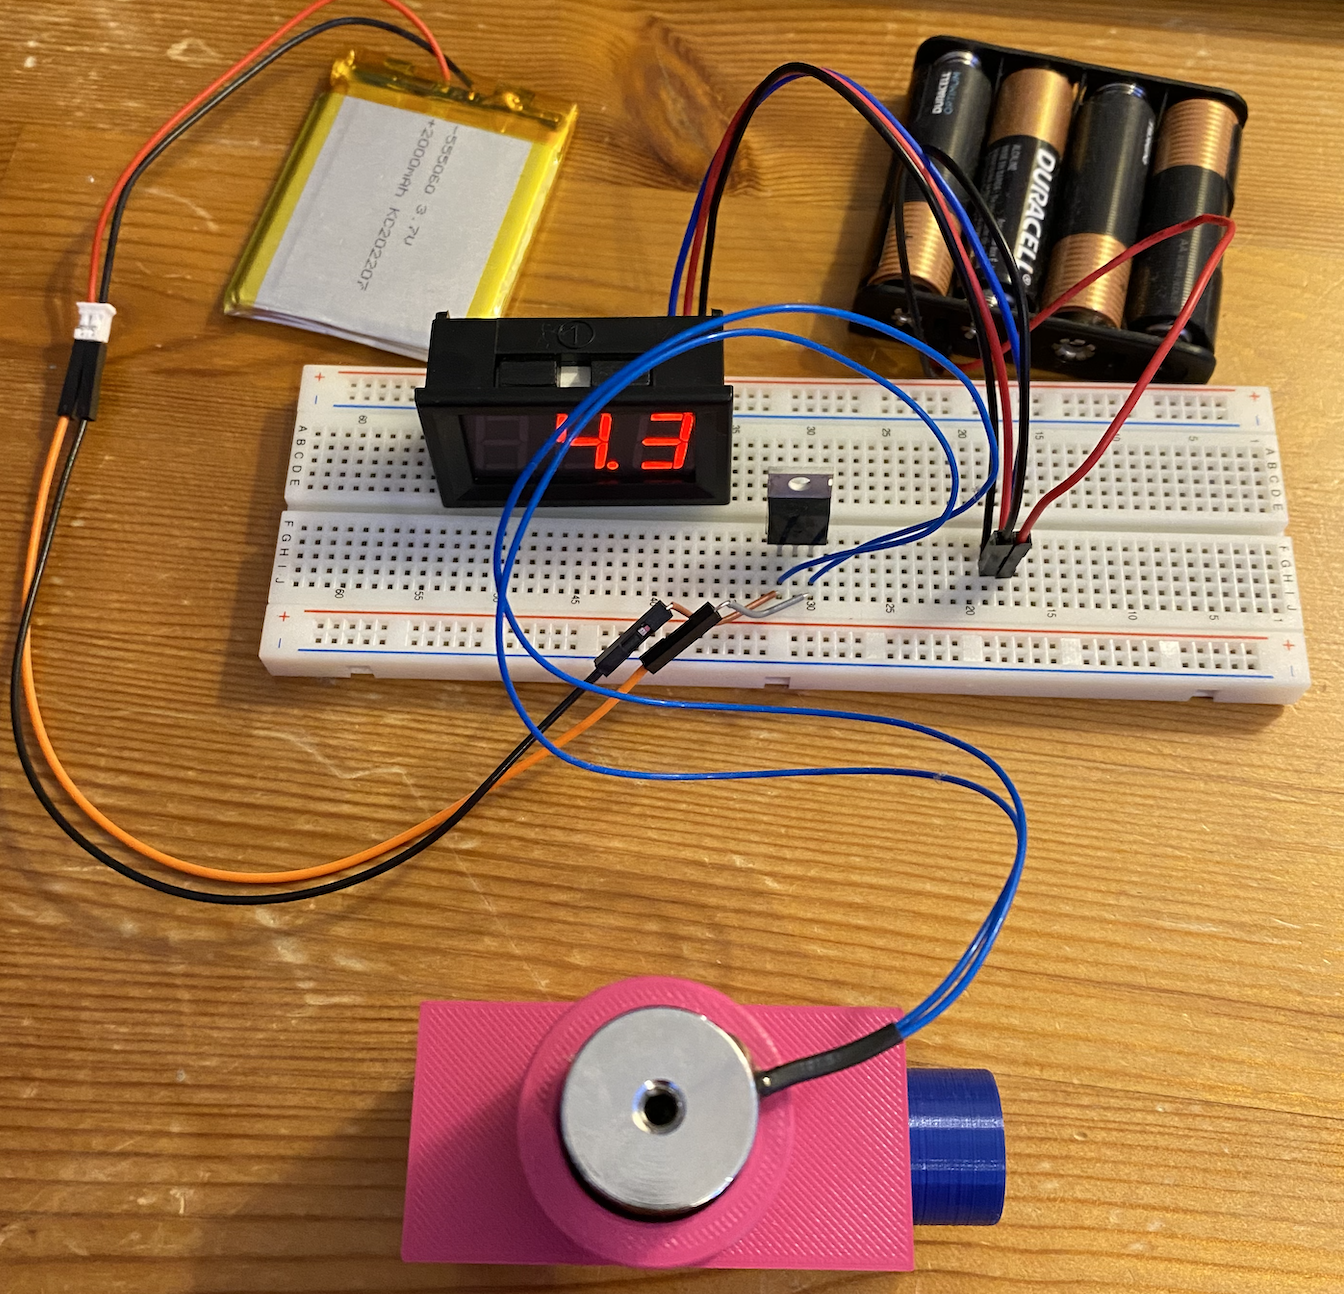
\includegraphics[width=0.5\linewidth]{6.png}
 }
 \caption{\label{Circuit} Circuit without the Arduino}
 \end{center}
 \end{figure}
 
  \begin{figure}[ht]
 \begin{center}
 {
  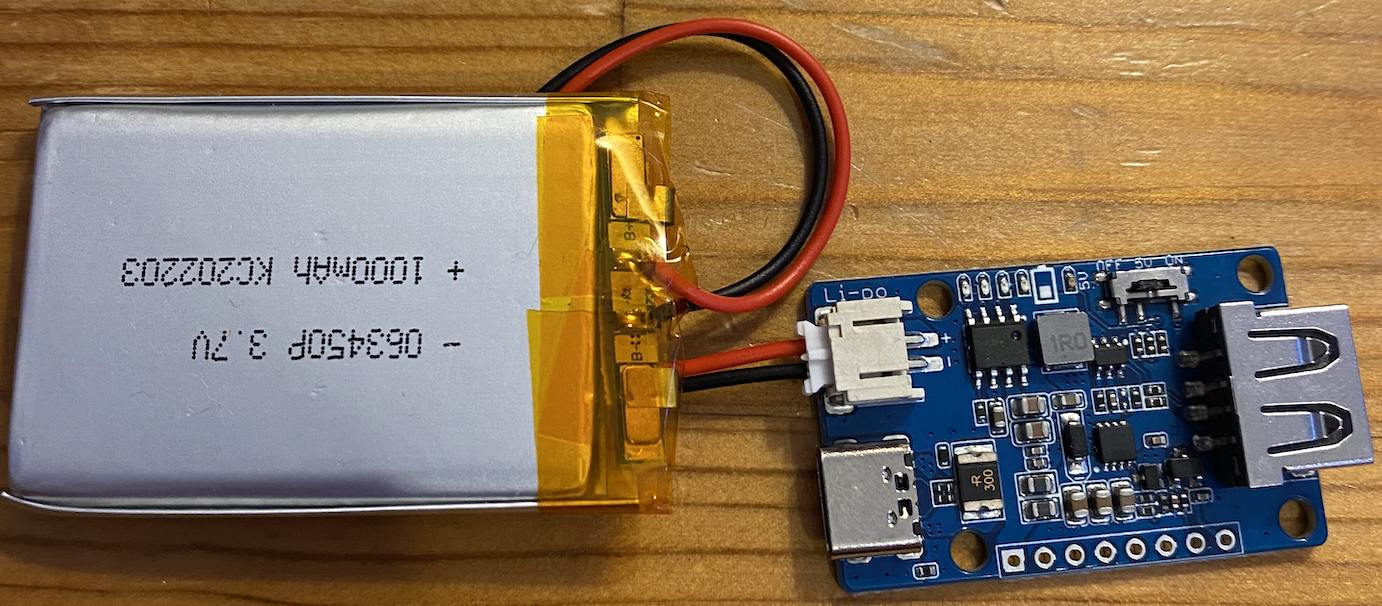
\includegraphics[width=0.5\linewidth]{8.png}
 }
 \caption{\label{Rechargeable Battery} Rechargeable Battery}
 \end{center}
 \end{figure}
 
 
  \begin{figure}[ht]
 \begin{center}
 {
  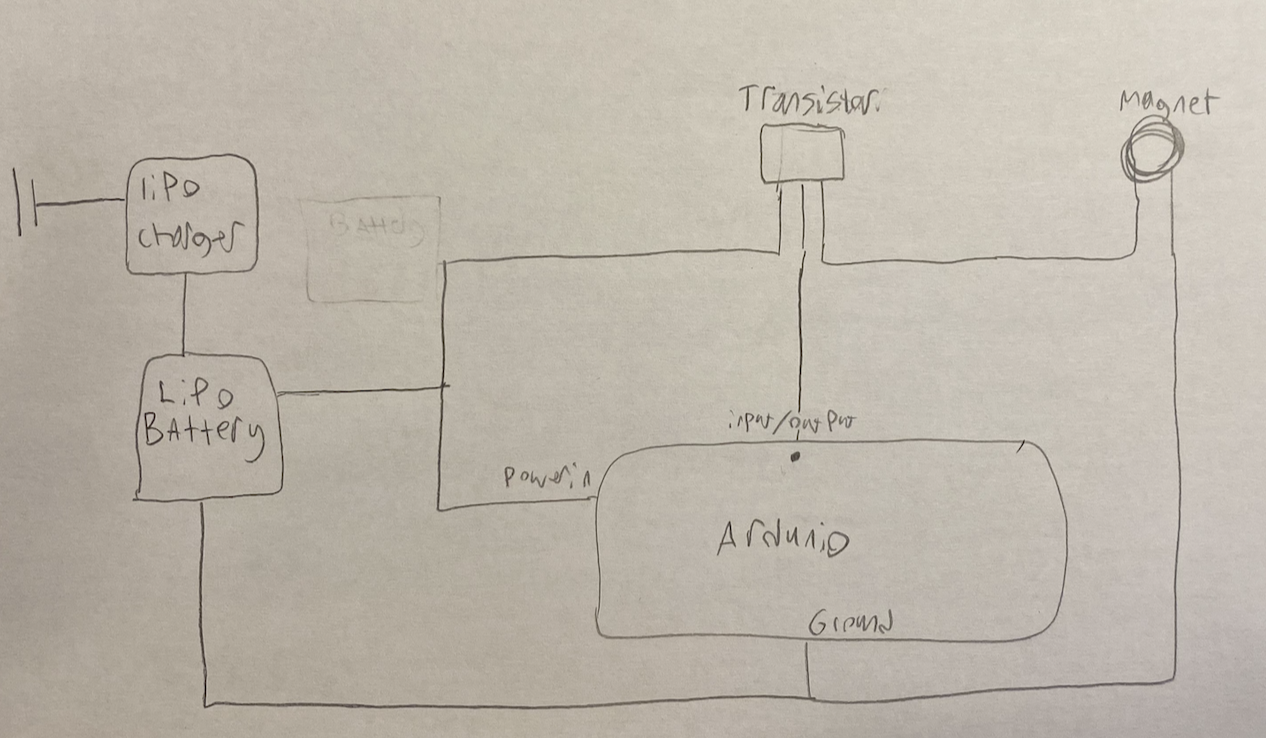
\includegraphics[width=0.5\linewidth]{10.png}
 }
 \caption{\label{Circuit Diagram} Circuit Diagram}
 \end{center}
 \end{figure}
 
 \newpage
    
 \newpage
 
\subsection{Communication Protocols - Included in Section 11}

%Communication protocols are if you are broadcasting or receiving messages.  If your project doesn't do this, then you don't need to worry about this section.


\subsection{Reflection}

The information in this section will be used to evaluate the team members on the
graduate attribute of Problem Analysis and Design.  Please answer the following questions:

\begin{enumerate}
  \item What are the limitations of your solution?  Put another way, given
  unlimited resources, what could you do to make the project better? (LO\_ProbSolutions)
  
  Given unlimited resources our bike lock would function without any human exertion, ie. mechanics, specifically, motors would work to open and close the lock eliminating the need for the user to touch the lock at all. They would simply have to touch a button on their phone. Additionally, there would be separate components to ensure the locking of the wheels to the frame and the frame to an external secure location.  Finally, with unlimited resources, there would be a way to ensure the seat of the bike could not be removed either.
  
  \item Give a brief overview of other design solutions you considered.  What
  are the benefits and tradeoffs of those other designs compared with the chosen
  design?  From all the potential options, why did you select documented design?
  (LO\_Explores)
  
  All of our solutions were fairly similar given that there are only so many different ways to lock a bike. The main differences came from various housing alternatives and "chain" variations. Our original idea functioned more similarly to the ideal situation described above, but in scaling our project to be realistic we had to eliminate and restructure our ideas.  
  
  Some of our other ideas were: 
  \begin{itemize}
\item A foldable chain that could be folded up small and compressed to the bike while riding
\item A circular arm for locking
\item An extendable arm so that you could be multiple distances
\item Individual locking units for each component
\end{itemize}

We landed on our final design because it uses components that are familiar to the average bike rider, it allows for the bike to be varying distances from a frame and it only involves one locking mechanism which is simpler, less bulky and easier to use. Additionally, we opted against the motor as a way to eliminate physical intervention because it would require much more battery and replacing or charging the battery that often would be more inconvenient than using your hands to insert the lock.


  
\end{enumerate}

\end{document}